% % % % % % % % % % % % % % % % % % % % % % % %


\documentclass[10pt,letterpaper]{article}
\usepackage[top=0.85in,left=1.25in,footskip=0.75in]{geometry}

%tikz packages for drawing grammar trees
\usepackage{tikz}
\usepackage{tikz-qtree}
\usetikzlibrary{positioning}

% amsmath and amssymb packages, useful for mathematical formulas and symbols
\usepackage{amsmath,amssymb}

% Use adjustwidth environment to exceed column width (see example table in text)
\usepackage{changepage}

% Use Unicode characters when possible
\usepackage[utf8x]{inputenc}

% textcomp package and marvosym package for additional characters
\usepackage{textcomp,marvosym}

% cite package, to clean up citations in the main text. Do not remove.
\usepackage{cite}

% Use nameref to cite supporting information files (see Supporting Information section for more info)
\usepackage{nameref,hyperref}

% line numbers
\usepackage[right]{lineno}

% ligatures disabled
\usepackage{microtype}
\DisableLigatures[f]{encoding = *, family = * }

% color can be used to apply background shading to table cells only
%\usepackage[table]{xcolor}

% array package and thick rules for tables
\usepackage{array}

% create "+" rule type for thick vertical lines
\newcolumntype{+}{!{\vrule width 2pt}}

% create \thickcline for thick horizontal lines of variable length
\newlength\savedwidth
\newcommand\thickcline[1]{%
  \noalign{\global\savedwidth\arrayrulewidth\global\arrayrulewidth 2pt}%
  \cline{#1}%
  \noalign{\vskip\arrayrulewidth}%
  \noalign{\global\arrayrulewidth\savedwidth}%
}

% \thickhline command for thick horizontal lines that span the table
\newcommand\thickhline{\noalign{\global\savedwidth\arrayrulewidth\global\arrayrulewidth 2pt}%
\hline
\noalign{\global\arrayrulewidth\savedwidth}}

% Text layout
\raggedright
\setlength{\parindent}{0.5cm}
\textwidth 5.25in 
\textheight 8.75in

% Bold the 'Figure #' in the caption and separate it from the title/caption with a period
% Captions will be left justified
\usepackage[aboveskip=1pt,labelfont=bf,labelsep=period,justification=raggedright,singlelinecheck=off]{caption}
\renewcommand{\figurename}{Fig}

% Use the PLoS provided BiBTeX style
\bibliographystyle{plos2015}

% Remove brackets from numbering in List of References
\makeatletter
\renewcommand{\@biblabel}[1]{\quad#1.}
\makeatother

% Leave date blank
\date{}

%% Include all macros below

\newcommand{\lorem}{{\bf LOREM}}
\newcommand{\ipsum}{{\bf IPSUM}}

%% END MACROS SECTION


\begin{document}
\vspace*{0.2in}

% Title must be 250 characters or less.
\begin{flushleft}
{\Large
\textbf\newline{Neural processing of sentences} 
}
\newline
% Insert author names, affiliations and corresponding author email (do not include titles, positions, or degrees).
\\
Amelia Burroughs\textsuperscript{*a}, %
%
% we need to ask Nina if she wants to be included; we could also include Tom Vaughan who made 
% the sentences; he needs to be in the acknowledgements anyway
% C 2018-08-13
%
% Tom Vaughan (? tbc), 
Nina Kazanina\textsuperscript{b}, %
%
Conor Houghton\textsuperscript{a}
\\
\bigskip
\textsuperscript{a}Computational Neuroscience Unit, School of Computer Science, Electrical and Electronic Engineering, and Engineering Maths, University of Bristol, UK\\
\textsuperscript{b}School of Psychological Science, University of Bristol, UK
\\
\bigskip

% Use the asterisk to denote corresponding authorship and provide email address in note below. 
* amelia.burroughs@bristol.ac.uk

\end{flushleft}
% Please keep the abstract below 300 words
\section*{Abstract}

% abstract: minor edits for typos
% C 2018-08-13

% abstact: very long, might try to shorten it a bit
% C 2018-08-13

How the human cognitive system is able to comprehend language has been
a matter of recent debate. 
%
%
On the one hand the brain may make use of
learned grammatical rules to decompose sentences into a hierarchy of
syntactic structures to generate meaning. On the other hand the brain
may rely on simpler, statistical methods where the generation of
meaning relies on sequential processing. 
%
%
Cortical activity has been
shown to track speech at the rate of syllable, phrase and sentence
presentation. This has been used as evidence for the language systems
ability to follow a rule-based grammar and generate a hierarchy of
linguistic structures during sentence comprehension. 
%
%
However, others
have suggested that the same results could be generated by a language
system that relies only upon sequences of word representations,
without the need for hierarchical phrase-structure building. 
%
%
Our goal
is to shed light on the extent to which hierarchical structure plays a
role in language processing during sentence comprehension. To this end
we use human EEG to record from participants as they listen to streams
of four word sentences. 
%
%
We confirm that cortical activity does
synchronise with the rate at which syllables, phrases and sentences
are presented. 
%
%
Sentence stimuli that contain both appropriate grammar
and semantic information generate a full brain response at the rate of
phrase presentation. This response is reduced if either grammar or
semantic information is absent. In sentences that lack both correct
grammar and meaningful semantics, the response at the phrasal rate
disappears. 
%
%
This suggests that both syntax and semantics are important
contributors during sentence processing, as opposed to just syntax
alone. 
%

\section*{Introduction}

% trimmed
% C 2018-08-14

% need to be clearer about the statistics based description
% C 2018-08-14
%% changed to defer any details of the two descriptions until later
%% C 2018-08-14

The ability of the human brain to rapidly generate meaning from an
incoming stream of sentences during natural language is
impressive. There are two competing, but not necessarily exclusive, theories describing how we are able to process words. Both
of these theories suggest that the smaller discrete units of language,
such as words and phrases, are concatenated by the brain into larger
units, such as sentences. What is under debate is the principles that
govern this organisation: one theory argues for the primacy of a
learned rule-based grammar, the other, for the primacy of statistical
relationships between the discrete units.

% In natural language use, words tend to occur in sequences. 
% removed and next sentence changed
% C 2018-08-13
%
% minor rewrite C 2018-08-13
%

In natural language the majority of utterances are composed of several
words that are put together in a sequence according to a set of
predefined rules that determine the serial order of language
elements. It is therefore of interest to understand how the brain
realises these rules. Linguists typically describe sentences in terms
of a hierarchical syntactic structure with a tree-like hierarchy of
nested phrases.

In support of this point-of-view, it has been demonstrated, using MEG
in \cite{DingEtAl2016} and using EEG in \cite{DingEtAl2017} that
cortical activity can entrain to the rate of syllable, phrase and
sentence presentation. In the EEG experiments participants were played
continuous streams of four-word sentences, where each word was 320 ms
long in duration and consisted of only a single syllable. As in
Fig.~\ref{fig:freq_tree} each sentence was composed of a noun phrase
and a verb phrase, which both contained two words. Thus these stimuli
have a specific frequency at three levels of linguistic structure:
syllables at 4/1.28 Hz, phrases at 2/1.28 Hz and sentences at 1/1.28
Hz. The neural responses were analysed using time-frequency
decomposition and measures of inter-trial phase coherence
(ITPC). Cortical activity was found to be phase-locked to the rate of
presentation of syllables, phrases and sentences even though only the
syllable frequency is present in the auditory signal itself, the other two
frequencies rely on the meaning of the words and the structure of the
sentences.  These results can be interpreted as evidence for neural
entrainment to discrete higher-level syntactic structures, as opposed
to neural tracking of, for example, transition probabilities during
sentence processing.

\begin{figure}[tb]
\begin{center}
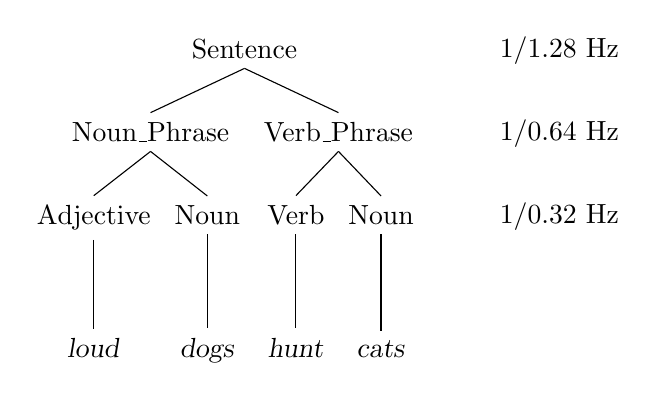
\begin{tikzpicture}
\tikzset{every tree node/.style={align=center,anchor=base}}
\tikzset{level 5+/.style={level distance=2\baselineskip}}
\tikzset{frontier/.style={distance from root=9\baselineskip}}
\Tree
    [.Sentence     
      [.Noun\_Phrase
        [.Adjective {\textsl{loud}} ]
        [.Noun  {\textsl{dogs}} ]
      ]
      [.Verb\_Phrase 
        [.Verb {\textsl{hunt}} ]
        [.Noun {\textsl{cats}} ]
      ]
    ]
 \node at (4,0.1) {1/1.28 Hz};
 \node at (4,-0.95) {1/0.64 Hz};
 \node at (4,-2.0) {1/0.32 Hz};
\end{tikzpicture}
\end{center}
\caption{Tree with frequencies \label{fig:freq_tree}}
\end{figure}

However, a considerable amount of behavioural data highlights the
significance of statistics during language comprehension. At the level
of word-statistics, word recognition times can largely be determined
by their frequency of occurrence in the language, word reading times
have been found to closely correlate with word probability and when an
ambiguous sentence has to be interpreted, the most probable
interpretation is most likely to be chosen (for review see
\cite{Jurafsky2002}). Additionally, both reading times and the
amplitude of neural responses are graded by the strength of
constraints imposed by prior context on possible sentence
continuations \cite{GibsonPearlmutter1998}. Language statistics must
therefore play a role in human language processing. 


In a statistical description, the brain, in a
Bayesian manner, exploits the rich statistical structure of language
to predict possible identities for syllables, words and phrases and
uses these predictions to aid the identification of the actual
linguistic input. In this picture, the interpretation of language
involves the production, reevaluation and resolution of predictions,
and grammar has evolved out of a kind of \lq{}language game\rq{} where
speakers aid each other by propagating conventions about how words are
arranged, enriching the statistical structure of utterances and syntactic categories are not psychologically real, but epiphenominal to a statistical based response to linguistic
stimuli.

In this context \cite{FrankYang2018} propose a computational model that
assumes no higher level of abstraction than a semantic
clustering of word representations. Their model represents each word
as a high-dimensional vector chosen so that the proximity structure of
the vectors matches the statistical relationship between the
corresponding words in a large language corpus. The frequency tagged
experiment from \cite{DingEtAl2016}, described above, were simulated
and the model generated power peaks at the same frequencies as those
observed experimentally. This suggests that the peaks could be
generated using only the lexical information within the word stimuli,
without the need for any knowledge of syntax. 

Here Electroencephalography (EEG) is used to measure responses to
simple meaningful sentences in comparison to sentences with two different
manipulations; nonsense sentences which have been deliberately chosen
to have little sensible meaning, and re-ordered sentences, in which
syntax has been destroyed by re-ordering the words. The aim of this
experiment is to help to distinguish between the two competing
explanations for the phrase- and sentence-level phase locking observed
in \cite{DingEtAl2016,DingEtAl2017}.

We used EEG to record neural activity while subjects listened to continuous streams of four single-syllable words that can combine to form a sentence consisting of a noun phrase and a verb phrase. We found that cortical responses become phase-locked to the frequencies at which syllables, phrases and
sentences are presented. A peak in the ITPC value is observed at the sentential rate (1/1.28 Hz). This is similar for sentences that are both grammatically correct and with semantically sensible words and sentences that are ungrammatical in terms of word order and contain semantically
 unrelated words. The peak in the ITPC value at the rate of phrase presentation
 (2/1.28 Hz) is maximal when sentences are both grammatical and make
 semantic sense. This peak is significantly reduced when either grammar or
 semantic sense alone is lacking and is absent when sentences are both ungrammatical and
 lack semantically-related words. 


\section*{Methods}
\subsection*{Participants}

Eighteen right-handed, native English speakers (11 female, mean age 26
years (range 22 - 32 years)) participated in this study. All
participants gave written, informed consent prior to undertaking the
study and were paid £20. Ethical approval for our experimental procedures were obtained from the University of Bristol Faculty of Science ethics board. All methods were performed in accordance with the relevant guidelines and regulations.

\subsection*{Stimuli}

The experimental procedures were similar to those used in a recent EEG
study (Ding et al., 2017). Listeners were played English sentences
composed of four single-syllable words. Each word was synthesised
independently using the MacinTalk Synthesizer (male voice Alex, in Mac
OS X 10.7.5). All of the synthesised words (226 - 365 ms) were
adjusted to 320 ms duration and volume normalised using the freely
available Praat software \cite{BoersmaWeenink2018}.

20 single-syllable words were chosen for each of the four word
categories: adjective, subject, verb, object. Words were selected if
they were synthesised clearly by the speech synthesiser and if they
could be easily categorised into a distinct word category.  This was
to avoid verbs, such as ride which can
often be used as nouns. Nouns were pluralised and all sentences were
played in the present tense.

Sentences were made by randomly selecting words from each of the four
word categories in the order 
\begin{quote}
adjective, subject noun, verb, object noun
\end{quote}
These sentences were then independently ranked in terms of how
much sense they made by 290 online participants recruited through
Prolific Academic. Participants were presented with 110 pairs of
sentences, ten of these were an attention trap; participant were asked
to press \lq{F}\rq{} in response to sentences containing the word
\lq{}fish\rq{} and were punished with a time out if they made a
mistake. For the remaining 100 pairs they selected the sentence which
\lq{}sounds more normal in everyday speech\rq{} (see supplementary
information for the full text of the participant instructions). Elo
chess ranking \cite{Elo1978} was used to derive individual scores for
each sentence from the pairwise comparisons. This established a
ranking from sense to nonsense. The top 20 sentences were chosen to form the
\lq{}sensical\rq{} sentence condition and the bottom 20 were chosen to form the \lq{}nonsensical\rq{}
sentence condition. 

Based on these sensical and nonsensical sentences four different conditions were created: the
original sensical sentences and nonsensical sentences along with two ungrammatical conditions in which the words for sensical and nonsensical sentences were re-ordered as
\begin{quote}
     verb, subject noun, object noun, adjective
\end{quote}
These four conditions are summarized in Table~\ref{tab:conditions}.

\begin{table}
\begin{tabular}{l|ll}
&sensible&nonsense\\
\hline\\
grammatical&\textbf{GS}: huge trams scare boys&\textbf{GN}: bored mugs write beds\\
ungrammatical &\textbf{US}: scare trams boys huge&\textbf{UN}: write mugs beds bored
\end{tabular}
\caption{A summary of the four conditions; the condition label used in the text is in
  bold, the sentence beside this gives an
  example.\label{tab:conditions}}
\end{table}

\subsection*{Experimental Procedures}

In total, 18 participants listened to 120 trials. For each of the four
conditions, 30 trials were presented. A trial was made up of thirteen
four-word sentences, played back to back in a continuous stream with
no acoustic gap between the sentences. Five trials were put together
to make a block. Each block consisted of five trials of the same
condition with an 800 ms break between trials. At the end of each
block participants were asked to rate the sentences on a scale of one
to five in terms of how much sense the sentences made to them on
average using a button press. Following the button press, the next
block was played after a delay of 1200 ms. Blocks were presented in a
random order and the order of the blocks was counterbalanced across
participants.

\subsection*{EEG Recording}

EEG was continuously recorded with a 32-channel EEG system (),
digitized at a sampling rate of 1,000 Hz (bandpass filter = 0.01–400
Hz) and referenced to the vertex (Cz), as in \cite{DingEtAl2017}. The
impedance of the electrodes was kept below 5kohms. Eyeblink artifacts were removed using ICA: an independent component
was removed if in its topography the mean power over the most frontal
three channels was more than twenty times stronger than the mean power
over all other channels. The signals of interest are in the
low-frequency region, at 1/1.28, 2/1.28, and 4/1.28 Hz and so the EEG
signal was lowpass filtered to 25 Hz. Data were referenced offline to
a common average reference and the responses to each individual trial
were epoched. 

\subsection*{Data analysis}

Upon sound onset there is a transient EEG response and
so the first sentence in each trial was removed from the data. This
meant that the overall trial length was 15.36 seconds (1.28 seconds x
12 sentences). The remaining EEG signal was converted into the frequency domain using the discrete
fourier transform with a frequency resolution of 0.065 Hz, that is, 1/15.36 Hz. The complex-valued Fourier coefficient of the trail $k$, $X_k(f)$, is then used to calculate the inter-trial phase coherence and the evoked power. 

The evoked power is
\begin{equation}
\label{eq:power}
E(f)=\left|\sum_k{X{_k}(f)}\right|^2 / K
\end{equation}
where $K$ is the total number of trials and  This value is
a function of frequency $f$. The evoked power reflects the power of EEG
responses that are timelocked to the auditory speech input. It is the
same as the power spectrum of the EEG response waveform averaged over
trials. The inter-trial phase coherence is defined in Eq.~\ref{eq:itpc}
\begin{equation}
\label{eq:itpc}
R(f)=\left(\sum_k{\cos{\theta_k}}\right)^2/K+\left(\sum_k{\sin{\theta_k}}\right)^2/K
\end{equation}
where $\theta_k$ is the phase angle of each complex-valued Fourier coefficient: $\theta_k = < X_k(f)$. As with the evoked power, it measures the timelocked response; because it uses only the phase-angle rather than the whole response, it does not show the same $1/f$ noise that is present in the evoked power.

For each trial, the mean alpha band frequency (8–12 Hz) power (as
calculated in Eqn.~\ref{eq:itpc}) over all channels was calculated and
correlated with the mean of the inter-trial phase coherence at the
phrasal frequency, 2/1.28 Hz. Linear regression analysis was used to
establish the correlation between inter-trial phase coherence at the
phrasal frequency and evoked alpha band power.

\subsection*{Significance Testing}

As in \cite{DingEtAl2016} a one-tailed paired t-test was used to test whether the inter-trial phase coherence value in a given frequency bin was significantly stronger than the average of the neighboring four frequency bins, two bins on either side. This was applied to all frequency bins below 5 Hz and a FDR correction for multiple comparisons was applied. 

A repeated measures, two-way ANOVA with a two (grammar: grammatical or ungrammatical) by two (sense: sensical or nonsensical) factorial design was performed to compare the main effects of grammar and sensible meaning on the strength of the ITPC at target frequencies across conditions. The TukeyHSD post-hoc test was used to compare the strength of the ITPC responses at different frequencies of interest (1/1.28 Hz, 2/1.28 Hz and 4/1.28 Hz) across each of the four conditions for all participants. p values of less than 0.05 indicate a statistically significant result.


\section*{Results}

Three significant peaks in the strength of the ITPC were observed in the EEG response at the sentential (1/1.28 Hz), phrasal (2/1.28 Hz) and syllabic (4/1.28 Hz) rates while subjects listened to four word sentences (Figure 3). These three peaks were significant in all of the four sentence conditions except for the peak at the sentential rate (1/1.28 Hz) in condition \textbf{GS}. In addition there is a statistically significant peak at 3/1.28 Hz in three out of the four conditions, which is likely due to be a resonance of the 1/1.28 Hz peak.

\begin{figure}[tbhp]
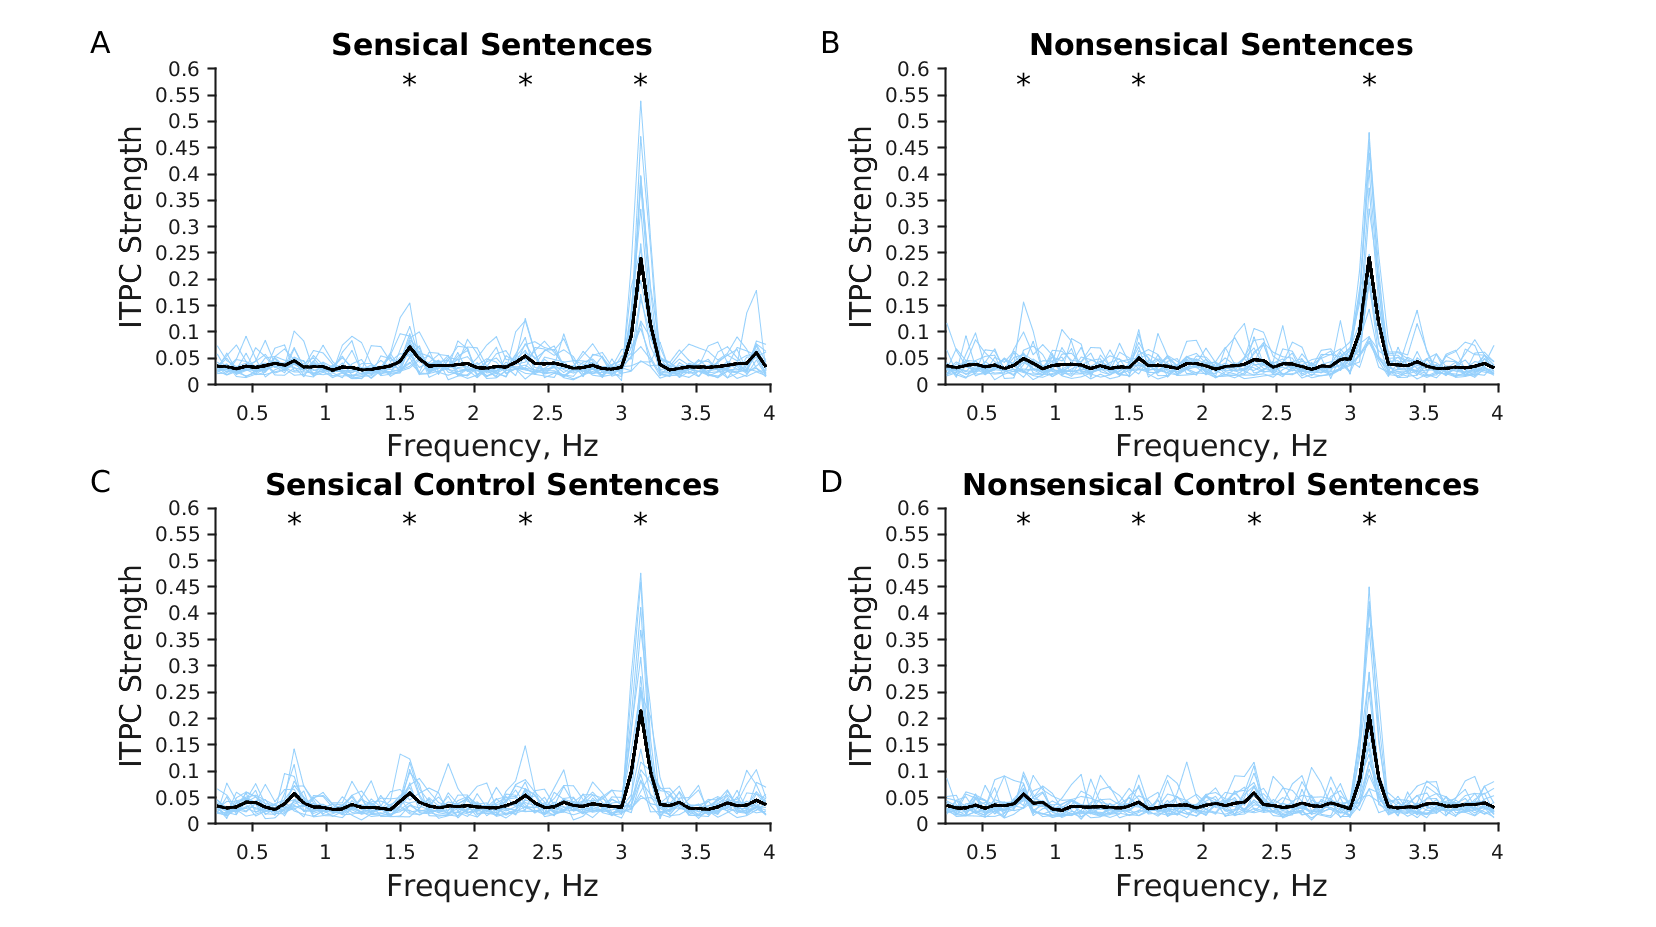
\includegraphics[width=\linewidth]{Grand_average_ITPC_per_condition_Grand_Average_ITPC_stats.png}
\caption{\textbf{The spectrum of inter trial phase coherence in the EEG response to sentences from each of the four conditions.} These figures show the grand average over all participants and electrodes to each of the four condition. Stars represent
statistical significance *= p$<$0.05, **= p$<$0.005, ***= p$<$0.0005.}
\label{Fig1}
\end{figure}

We first analyzed whether there were significant main effects of grammar and meaningful semantics on the strength of the inter-trial phase coherence at each of the three frequencies of interest in the EEG response (1/1.28 Hz, 2/1.28 Hz and 4/1.28 Hz), Figure 4. At the rate of phrase presentation (2/1.28 Hz) there was a significant main effect (Figure 4B) of both grammar (p=0.0096, F=8.4985, n=18 Subjects, mean(grammatically correct) =  0.0609 +/- 0.0293, mean(grammatically incorrect) = 0.0498 +/- 0.0291) and semantics (p=0.0025, F=12.5283, n=18 Subjects, mean(semantically related words) = 0.0648 +/- 0.0328, mean(semantically unrelated words) = 0.0459 +/- 0.0226). Both correct grammar and sensible semantics were associated with a significantly greater peak in ITPC strength at the phrasal rate than sentences with incorrect grammar or semantically unrelated words. No interaction effects were observed (p=0.7530).

At the syllabic rate there was a significant main effect of grammar (Figure 4C). The ITPC peak at the syllabic rate was significantly greater when participants listened to grammatically correct sentences compared to when the same participants listened to grammatically incorrect sentences (p=0.0016, F=14.0673, n=18 Subjects (mean ITPC at 1/1.28 Hz in the grammatically correct conditions = 0.2402 +/- 0.1434, mean ITPC at 1/1.28 Hz in the grammatically incorrect conditions = 0.2096 +/- 0.1381)). No significant main effect of semantics was observed (Figure 4C). At the rate of sentence presentation no significant main effects on the strength of ITPC were observed (Figure 4A).


%% include figure here detailing main effects results from repeated measures 2 way ANOVA.

\begin{figure}[tbhp]
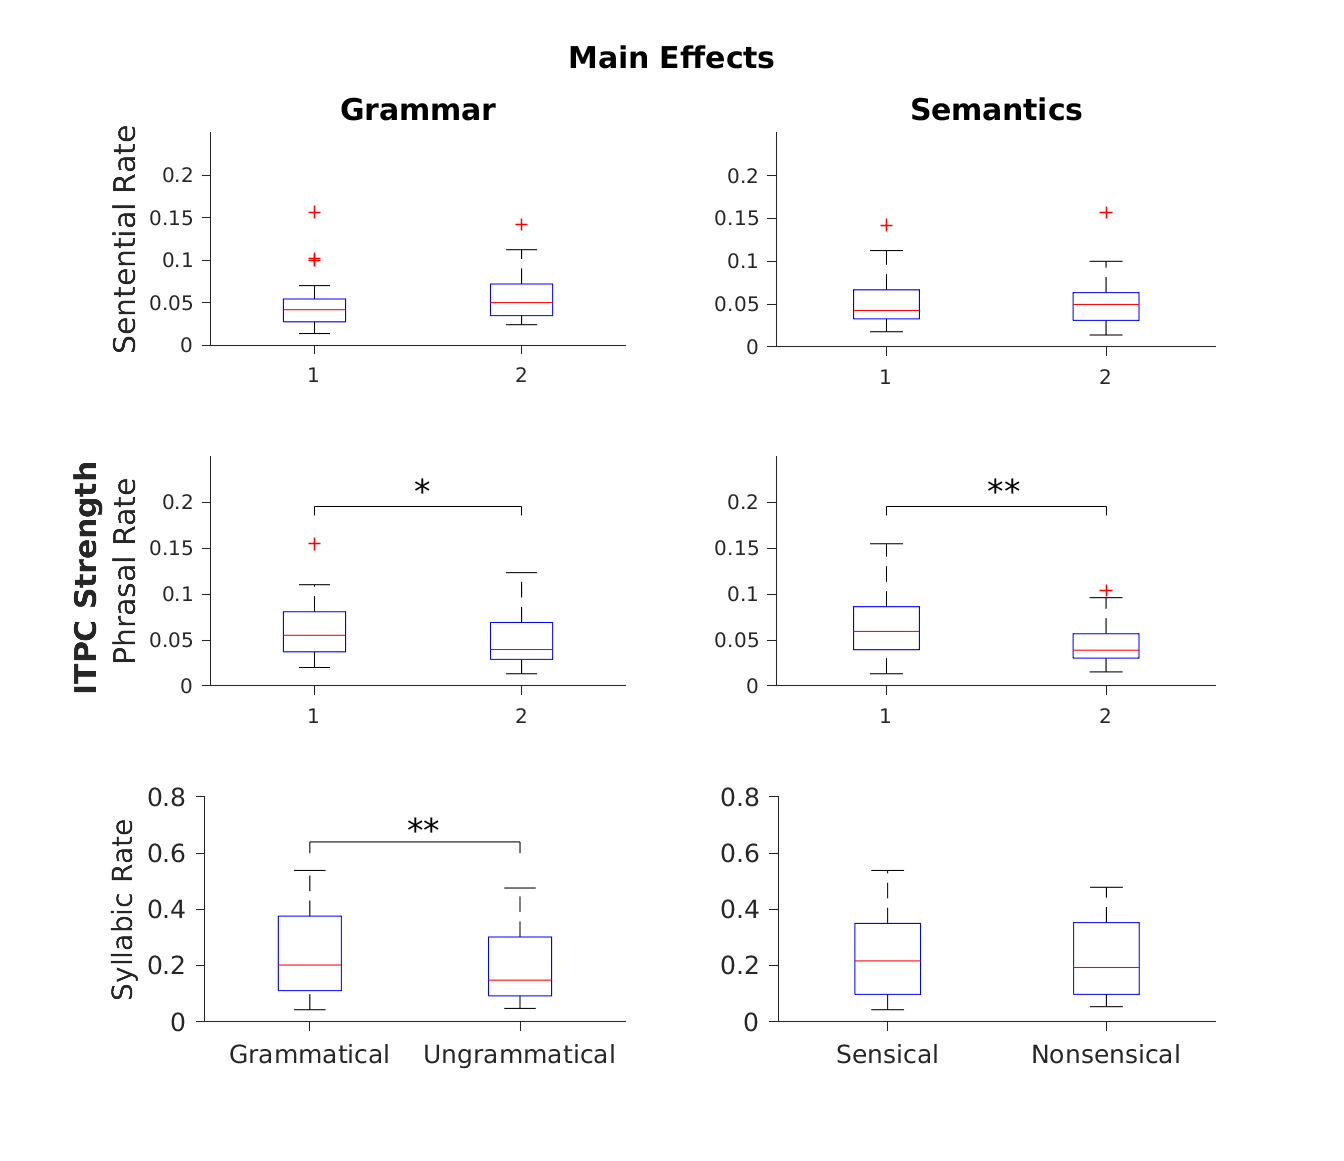
\includegraphics[width=\linewidth]{BoxPlots_main_effects.png}
\caption{\textbf{Main effects from the repeated measures 2-way ANOVA.} The main effects of grammar and sensible semantics on the strength of the ITPC at each of the three target frequencies of interest (1/1.28 Hz, 2/1.28 Hz and 4/1.28 Hz). A statistically significant effect of grammar was observed at both the phrasal and sentential rate, with a greater ITPC peak for grammatically well-formed sentences. A main effect of semantics was also observed at the phrasal rate. No interactions between grammar and semantics are present. Statistical significance *= p$<$0.05, **= p$<$0.005, ***= p$<$0.0005.}
\label{MainEffects}
\end{figure}

% now talk about pair wise comparisons across 4 conditions

The ITPC response at both the sentential and syllabic rate was similar across all of the four conditions (Figure 5A, 5C). We next compared the strength of the ITPC at the rate of phrase presentation between each of the four experimental conditions (Figure 5B). The strength of the ITPC at the phrasal rate is statistically significantly greater in response to grammatically well-formed, semantically sensible sentences in  condition \textbf{GS} (mean = 0.0712 +/- 0.0309) compared to both condition \textbf{GN} (p = 0.0328, mean = 0.0507 +/- 0.0242) and condition \textbf{UN} (p = 0.0015, mean = 0.0411 +/- 0.0205). No other comparisons were significant. Fig.~\ref{PhraseITPC} shows this comparison along with the participant-to-participant variation.

\begin{figure}[tbhp]
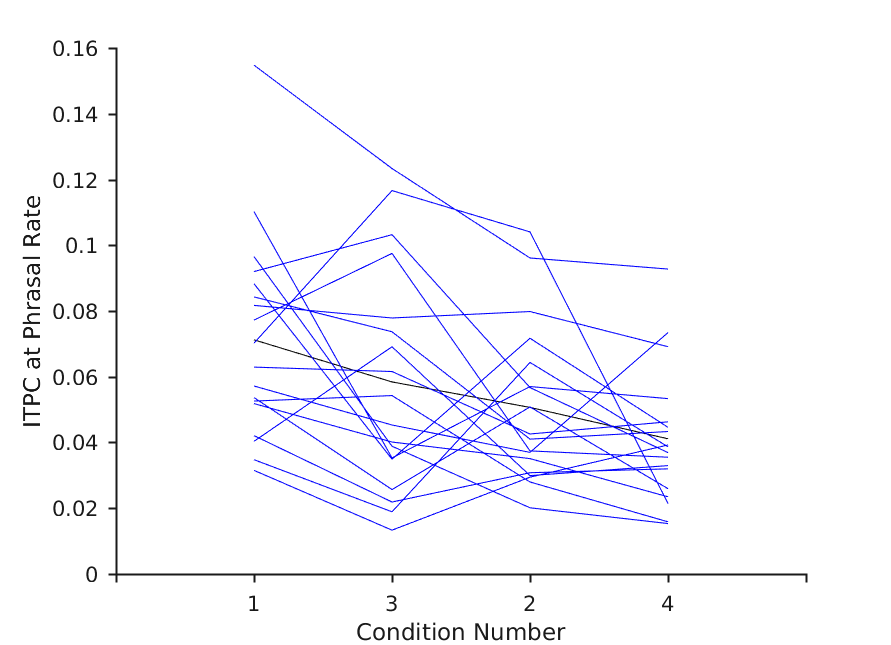
\includegraphics[width=\linewidth]{ITPC_peak_joined_for_participant_ordered_conditions_phrase_phrasal_rate.png}
\caption{\textbf{ITPC strength at the phrasal rate for each subject during each condition.} Graph showing the strength of the ITPC at the phrasal rate for each subject during each of the four experimental conditions. Each blue line represents a single subject. The black line represents the average ITPC strength at the phrasal rate for each of the four conditions across subjects.}
\label{PhraseITPC}
\end{figure}




\begin{figure}[tbhp]
%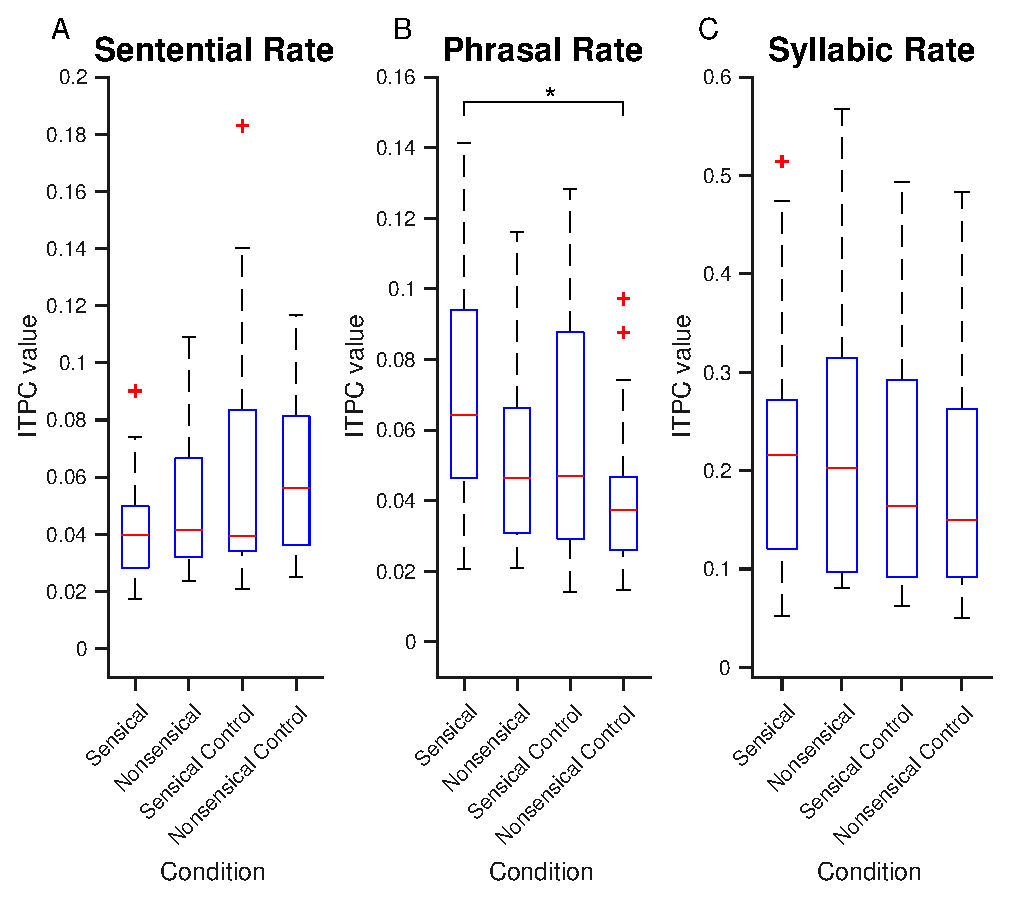
\includegraphics[width=\linewidth]{Figure3.eps}
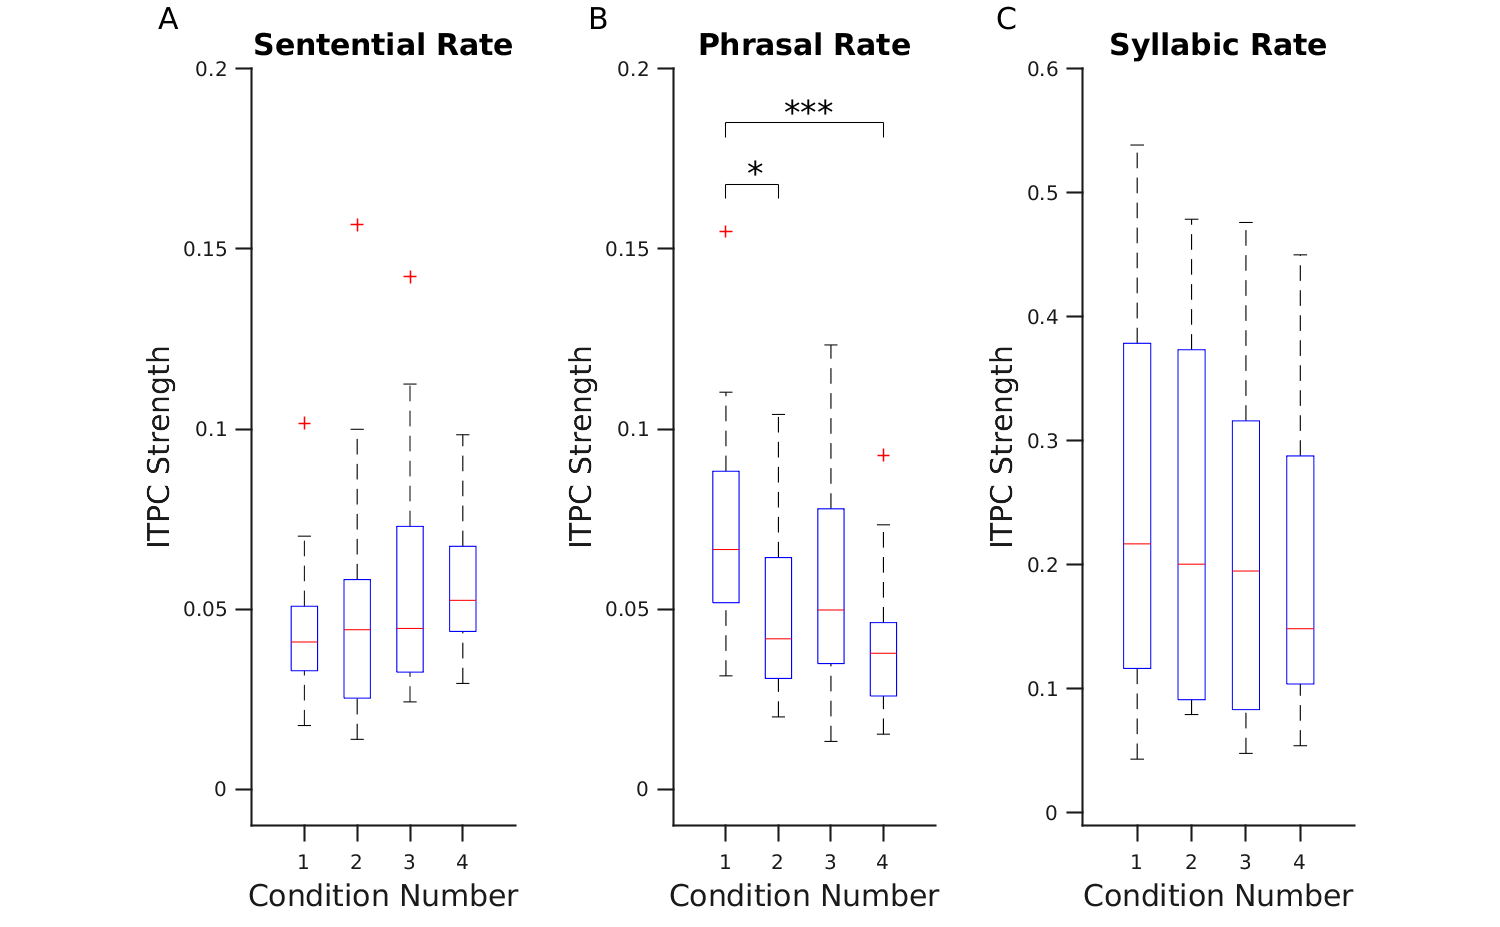
\includegraphics[width=\linewidth]{ITPC_peaks_per_condition.png}
\caption{\textbf{Comparing ITPC values at frequencies of interest
    across conditions} Graphs showing average ITPC values at the
  sentential, phrasal and syllabic rates (\textbf{(A-C)}; 1/1.28 Hz,
  1/0.64 Hz, 1/0.32 Hz, respectively) for each of the four conditions
  tested. On the box plots the the central red line indicates the
  median ITPC value for each condition at each of the target
  frequencies \textbf{(A-C)}, the bottom and top edges of the box
  indicate the 25th and 75th percentiles of the ITPC values,
  respectively. The whiskers extend to the most extreme data points
  not considered outliers, and the outliers are plotted individually
  using the '+' symbol. Stars represent statistical significance *=
  p\<0.05, **= p\<0.005, ***= p\<0.0005. The ITPC at the phrasal rate was
  significantly greater when subjects listened to grammatically
  correct, semantically plausible sentences (condition 1) than when the same
  subjects listened to sentences that were either formed from grammatical,
  semantically unrelated words (condition 2) or from ungrammatical,
  semantically unrelated words (condition 4).}
\label{ITPC_peaks}
\end{figure}


% outline variability in participant results


% add graph for individual subject ITPC peaks in each condition at phrase rate 






% add in a sentence to state effect of time and condition order and phase
No effect of time was observed in the present study (see Supplementary Material). The ITPC graphs were similar when comparing trials that occurred at the beginning of each experiment compared with trials that occurred later, and when comparing the responses to sentences that were presented during the first half of each trial with the last half of each trial. In a number of cases where conditions \textbf{US} and \textbf{UN} were presented to participants before either conditions \textbf{GS} or \textbf{GN}, the peak in ITPC at the 1/1.28 Hz rate was still evident. Therefore, the peak observed in ITPC at the sentential rate to presentation in the ungrammatical conditions were not the result of the expectancy of four word sentences given by the prior presentation of sentences from the grammatical conditions. 







\section*{Discussion}

% this is too long; we need to cut it down, but
% make sure we save the origin since it has lots of 
% good stuff in it.
% C 2018-08-14

We used EEG to record cortical activity in response to sentences
composed of four single-syllable words that can combine to form a noun
phrase and a verb phrase. We found that neural responses become
phase-locked to the frequencies at which syllables, phrases and
sentences are presented. This is inline with both MEG and EEG
recording studies of sentence processing.
\cite{DingEtAl2015,DingEtAl2017}. The main findings from this study
are that:
\begin{itemize}
\item A peak in the ITPC value is observed at the sentential rate
  (1/1.28 Hz). This response is similar for sentences that are both
  grammatically correct and contain words which combine to give
  meaningful semantic information and sentences that are both
  ungrammatical in terms of word order and contain semantically
  unrelated words
\item The peak at the rate of phrase presentation
  (2/1.28 Hz) is maximal when sentences are both grammatical and make
  semantic sense, absent when the sentences are both ungrammatical and
  lack semantically-related words and reduced when either grammar or
  semantic sense alone is lacking. 
\end{itemize}
%
% 
% I think this is worth pointing out
% C 2018-9-17
%
It is notable that the sentence peak (1/1.28 Hz) does not differ
across conditions, but the phrase peak (2/1.28 Hz) is significantly
different between conditions one and four and one and two. This indicates that the
phrase peak cannot be explained as a resonance of the sentence peak.

% paragraph break
% C 2018-9-17
%
% need to think about this
% 
% grammar and sense not needed for sentence peak
% phrase peak requires both grammar and sense
% this does seem to support statistical rather than hierarchy,
% how clearly do we want to claim that
% C 2018-08-14
%
These findings combine to suggest that language is most likely
processed in terms of sequences of word representations. Our findings
also suggest that semantic information may play a considerable role
during natural language comprehension and syntax may not in fact be
the primary driver of comprehension as is often suggested.

The presence of an ITPC peak at the sentential rate, even in the
absence of syntactic information or semantically related words, is
indicative of statistical processing at the word-level driven by
syntactic category information. 
%
%
%
% one complication is that the condition 1 sentences might
% create the expectation that these are suppose to be four word 
% sentences, is the block order the same for all participants
% are there any where there is a condition 3 or 4 block first?
%
%% We have 5 subjects that get between 5 and 10 trials of either condition 3 or 4 before wither of conditions 1 or 2 and you still see a substantial peak at 1/1.28 in the majority of these subjects
% Add in a line about this to the text
%% A 2018-08-22
%
% alternatively is there a change in the effect from early blocks to 
% later blocks?
%
% C 2018-08-14
%
%% No observable change
%% Make a nice figure to illustrate this
%% A  2018-08-22
In experimental conditions \textbf{US} and \textbf{UN}, the four-word sentences are
ungrammatical and do not consitute well-formed sentences. The only
information that occurs at the sentential rate is therefore the
repetition of words that share a common syntactic category at the same
position across sentences. For example, a verb is repeated every four
words. The peak at the sentential rate must therefore be driven by the
repetition of an adjective, verb, subject and object at the first,
second, third and fourth position in every sentence presented.
%
%
% this is complicated; verbs are a category, they are also a set
% of words that have something in common because they are all 'action words'
% what do Frank and Yang say when making their origin prediction?
% C 2018-08-14
%
%
% another interpretation of all this is that the appearance of another
% verb closes off any predictions about there being a sentence
% so what we are see is 'well I guess that wasn't a sentence'
% signals
%
% this idea could be made to fit with a hierarchical approach
% it marks the collapse of an attempt to construct a tree
% this doesn't seem likely but we should mention it?
%
% C 2018-08-14
%
%

The results presented here show that sentences are most likely
processed in a sequential manner determined by word-category
statistics. 
%
%
 This is supported by the fact that the occurrence of a
particular word does not usually allow for good prediction of the
words that follow it. As Pulvermuller, 2002, states, it is likely that
the regularities governing word sequencies likely operate over lexical
category. This means that the presentation of a pronoun for example
can predict, with high probability, the later occurance of a
compliment verb. For this to be possible abstraction over word category is
necessary. Our results presented here are inline with this
theory. 
%
%
This is in line with modern grammars, which tend to be lexical in
nature. As such, much of the knowledge necessary for sentence
structure is stored in the lexicon with the individual words,
alleviating the need for this to be computed by abstract hierarchical
phrase-structure rules. At least in the conditions presented in this
study. It is quite probable that a more complicated set of rule-based
analyses may be relied upon during more complex linguistic analysis,
but that statistical-based analyses are preferred during simple, every
day language situations. 
%
%
% this raises the question, do we see a higher N400 for our nonsensical
% sentences? maybe the is too hard to see with everything else going on?
% C 2018-08-14
%
% *
% more speculatively, if we give a N400 for every word, but make is smaller
% for expected words, do we recapitulize the EEG results?
% this would be easy to check! Also hilarious if true!
% C 2018-08-16
%

% to elaborate, make a pretend N400, maybe a little piece of cos
% centred on 400 ms about 75 ms wide add one of these every 0.32 ms
% with a variable amplitude, say noisy but either h or l and then try
% streams that look like hlhlhlhlhlhlhl and hhhhhhhhhh and
% hllLhllLhllL where L is lower than l and run these fictive traces
% through the same analysis as the real data!
% C 2018-9-17
%
%
In the ERP literature, the size of the N400 neural response can be
predicted to a higher degree of accuracy when the conditional
probability of a word is is estimated using an n-gram model as opposed
to a model of hierarchical phrase-structure grammar. The N400 response
may too follow word-probabilites. This supports the importance of
statistical processing during language use.

%  so with chuncks the crucial question, what is a chunk; how does the
% brain decide what a good chunk is? what is our story for what
% happens from the pov of chunking in the different cases?  
% C 2018-08-14

% I'm having trouble understanding how chunking relates to predition,
% trying to rewrite the paragraph to emphasise this.  perhaps we
% should have some sort of reading group for the
% ChristiansenChater2016 paper!
% C 2018-08-16

%Another idea in regards to language processing has been put forward by

In \cite{ChristiansenChater2016} it is argued that the key to
understanding the relationship between language and language
processing is to consider how serial processing of linguistic input
can occur despite the relatively small capacity of short term memory
and the long-range global dependencies present in language. Central to
their description is \lq{}chunk-and-pass\rq{}, the aggregating and
translating of sequential elements. This chunk-and-pass operation
occurs at multiple levels going from phonemes to words, words to
phrases, phrases to clauses and so on; the key idea is that in
linguistic processing, whenever possible, sets of sequential units are
translated into a unit with a more abstract representation. For the
\lq{}chunked\rq{} representation to be more compressed than the units
it replaces, there should be some dependency between these
units.

% provisionally commented out
% C 2018-08-16
%
%%  who argue that language input is
%% rapidly recoded by the brain into chunks. These chunks can then be
%% passed on to higher levels for further analysis. Chunking is driven by
%% the language system's ability to learn to process, rather than induce,
%% grammar. Chunks are built up incrementally and involve greater and
%% greater levels of linguistic abstraction, into which input can be
%% continually recoded. Under this scheme prediction plays a substantial
%% role, allowing chunking to occur as early as possible and in parallel
%% across different levels and at varying timescales. Christiansen and
%% Chaser argue that the interpretation of the grammatical nature of
%% words in a sentence occurs via incremental processing, which also
%% relies on the linear order of words. 
%% %
%% They suggest that sequential word
%% processing, as opposed to hierarchical phrase-structure building,
%% plays an important role in explaining many grammatical phenomena. And,
%% although chunk-and-pass processing induces a multilevel structure over
%% linguistic input, it is driven by word order predictions as opposed to
%% learned hierarchical syntactic rules. This proposal fits in well with
%% research into working memory capacity and explains our ability to
%% percieve speech sounds at a much fast rate than nonspeech sounds
%% (Warren et al., 1969). 
%
% not sure what this means
% C 2018-08-14
%
%Language statistics are also essential for
%explaining the efficiency with which we are able to comprehend
%language and its robustness against errors and ambiguity.

The findings presented here are consistient with this chunk-and-pass
description of language processing; in condition one the sentences
fall into natural chunks based on the syntax of the sentence, these
chunks are readily represented abstractly because the constituent
words for meaningful phrases and the process of chunking is aided by
the semantic regularity of the sentences. For condition four all these
elements are absent and the lack of a phrase peak in the ITPC perhaps
indicates that no chunking occurs at the phrase level. From the
perspective of chunk-and-pass it is perhaps surprising that there is a
phrasal peak for condition three, composed of re-ordered sensical
sentences; these sentences should lack any phrasal structure, however,
it would appear that the semantic relatedness of some proximal words
is sufficient for some chunking to occur at the phrase rate. This
suggests that semantics plays an important role in the comprehension of
spoken sentences.

% provisionally commented out
% C 2018-9-17
%% Words tend to be processed in a statistical manner, but once words
%% combine to form a meaningful phrase, phrases get chunked and are
%% prepared for later combination into sentences. Both sensible grammar
%% and sensible semantic information is necessary for phrases to be
%% constructed from the incoming speech stream. In this condition
%% (condition one), a maximal ITPC peak at the phrasal rate is
%% generated. If either accurate syntax or meaningful semantics missing,
%% a phrase remains unresolved and the ITPC at the rate of phrase
%% presentation is reduced. This suggests an important, and often
%% overlooked, role for semantics in language processing. If both
%% grammatical information and semantic information is lacking (as in the
%% nonsensical control condition) then the ITPC peak at the rate of
%% phrase presentation is absent. Our study therefore suggests that both
%% correct syntax and meaningful semantics are both necessary to generate
%% a full brain response in listeners hearing sentences. The differences
%% observed between the ungrammatical sentences presented in conditions
%% three and four (formed from words making up sensical and nonsensical
%% sentences respectively) must be due to differences in terms of
%% semantic processing as the grammar remains the same. The phrase
%% response may be due to the fact that the words in condition three do
%% that tend to occur together in phrases in natural language and so each
%% word may result in more robust, overlapping and longer-lasting neural
%% representations than words that do not tend to co-occur. Therefore a
%% response at the rate of phrase presentation can be generated even if
%% the syntax used to combine the words into phrases and sentences is
%% incorrect, so long as the words are semantically related. We therefore
%% suggest that semantics plays an important role in the comprehension of
%% spoken sentences.

% small edits 
% C 2018-9-17

In a recent intracranial recording study reported in
\cite{FedorenkoEtAl2016} neural activity was recorded from the surface
of the brain while participants read sentences. Sentences consisted of
eight words and were either of a sensical form whereby word meaning
and grammar were correct, a \lq{}Jabberwocky\rq{} form where sentences were
well structured grammatically but had no overall sensible meaning, or
a word list form with no syntactic structure. A fourth condition was
non-word lists. Gamma-power was used to index neural activity, and was
found to increase monotonically over the course of an entire sentence
as it was read by the participant. This increase was absent in
non-word lists. In response to Jabberwocky sentences and word-lists
with the same word length the monotonic increase in gamma-power was
still evident, but to a lesser degree than when participants read
sensible sentences. As in the experiment reported here, this seems to
indicate that the increase in gamma power observed in response to
sensible sentences could not be explained by either word meaning or
syntax alone and that sentence understanding is a compositional
process. The construction of linguistic meaning may rely on both
semantic and syntactic interpretation.

It is possible that syntax and semantics can overlap to a certain
degree. \cite{Pulvermuller2002} suggests that the brain's responses to
words reflect both word semantics and lexical status;
\cite{KempsonEtAl2016} go further and suggest that syntax relies on
the incremental building of semantic representations. The experiment
reported here suggests that both correct syntactic and predictable
semantics need to occur together to generate a full brain response
during sentence comprehension. 

% maybe too directly argumentative!
% C 2018-9-17
%
%This is in contrast to Ding et al.,
%2016 who state in their introduction that linguistic structure
%building can occur purely because of the listener's grammatical
%knowledge and argue that larger linguistic structures are generated
%internally by necessity in a manner dependent upon syntax.  Our
%results suggest that statistical cues regarding a combination of
%syntactic and semantic information are both critical to sentence
%processing.

% all good stuff, but the dicussion is very long so commented out
% C 2018-9-17

%% Nelson et al., 2017 also recorded intracranially from epileptic
%% patients while they read sentences word-by-word. They found that high
%% gamma power increased with each successive word, but when a word could
%% be combined into a phrase, gamma power suddenly decreased. This
%% provides evidence for a merge operation carried out by the brain, in
%% which words are merged into phrases. They used model comparison to
%% show that sequential word processing over lexical and syntactic
%% categories could explain activity in the posterior middle temporal
%% gyrus, whereas hierarchical models are necessary to capture activity
%% at other sites within the superior temporal gyrus and inferior frontal
%% cortices. Like in Federenko et al., 2016 they found that each
%% additional word contributes similar amounts of additional neural
%% activity, but Federenko et al., did not observe the sudden decrease in
%% gamma power on appearance of a word that could be merged into a
%% phrase. This may be due to the type of probes that were used in the
%% two studies. In Nelson et al., 2017 the participants read an elliptic
%% probe presented 2.2 seconds after each sentence and were asked whether
%% it matched the previous sentence, for example 'he did' compared to
%% 'they should'. This probe therefore required patients to commit the
%% phrase-structure of the sentence to memory, which could well force
%% them to process the sentence hierarchically. Federenko et al., 2016 on
%% the other hand present only a single word at the end of each trial and
%% participants had to decide whether or not the probe word occured in
%% the preceding sentence. These differences may drive different levels
%% of processing and underlie the differences in the response patterns
%% observed in these two studies. This may possibly elude to that fact
%% that people can implement both sequential and hierarchical processing
%% mechanisms and drive language comprehension.

%% This fits in with the idea proposed by Frank et al., 2002 who suggest
%% that people are capable of processing both sequentially, in terms of
%% word level statistics, and hierarchically. The choice as to which
%% processing scheme is employed would depend on the complexity of the
%% sentence, and the context, but the most simple would often be
%% preferred. Language users can often rely on prababilistic knowledge
%% about upcoming words or syntactic categories of words, given the
%% preceding sequence of words they have already
%% encountered. Furthermore, the idea of sequential processing fits well
%% into our understanding of how the brain works. As suggested by Frank
%% and Yang (2002, 2018a, 2018b) a hierarchical account would not adhere
%% to the principles of free energy.

% doesn't fit so well with out story
% C 2018-9-17

%% In terms of a neurophysiological understanding of the brain mechanisms
%% involved in sequential processing it is possible that groups of
%% neurons work together to act as a sequence detector and detect
%% sequences of words that are likely to occur together. These neurons
%% would be fed information from neural networks involved in processing
%% word representations. Studies have shown that distributed populations
%% of neurons are activated by words, and not pseudo-words, and that word
%% presentation activates functional neural networks with multiple, fast
%% reverberatory loops. These circuits appear to be topographically
%% organised so that words relating to different word categories, for
%% example nouns and verbs, show differential topographic
%% representations. Neuroimaging studies give evidence to suggest that
%% different brain processes are involved in the processing of nouns
%% compared to verbs. Evidence suggests that semantic, as well
%% grammatical, properties of words are critical for determining specific
%% word-category brain responses. For example, visually-related nouns
%% evoke a differential brain response to action-related verbs, whereas
%% no difference in the topography is observed in the neural response
%% patterns evoked by nouns with strong action-associations, and
%% action-verbs (Pulvermuller, 1999). Similar results have been found
%% across a number of different modalities (Pulvermuller et al., 1999b
%% and Kiefer, 2001).

%% The idea that language might be processed by sequence detectors has
%% been put forward by Pulvermuller, 2002, who argues that word-sensitive
%% sequence detectors may be sensitive to sequences of words from
%% discrete categories. The occurance of a word from one particular
%% category may predict the later occurance of a word from another
%% word-category. The sequence detector could learn to become sensitive
%% to activation by a sequence of elements from different groups, for
%% example a pronoun followed by a complement verb. This would allow for
%% generalisation from a limited sample to novel, unheard sequences of
%% words when encountering previously unheard sentences. Neurons acting
%% together as sequence detectors are necessary in other domains such as
%% during the viusal detection of movement direction. The brain is good
%% at detecting sequences and many behavioural studies have shown that
%% sequence detection tasks, such as identifying the pattern of musical
%% notes when listening to music, recruit similar, overlapping brain
%% regions to language. Sequence detectors can allow for variable time
%% delays that may last on the order of several seconds. This would be
%% necessary in the context of language where there are often long
%% delays. Inline with ideas reporting that human syntax is processed by
%% a sequence processor, hidden Markov models and simple recurrent
%% networks are sequence learning mechanisms that have been shown to be
%% capable of acquiring syntactic knowledge and are able of simulating
%% human grammatical behaviour. Furthermore, theories of sequential
%% processing of language are able to account for the principles of
%% linguistic agreement, which is the relationship between a
%% sentence-initial pronoun and a sentence-final suffix, which need to
%% agree in terms of both number and person. Hierarchical accounts of
%% sentence structure that involve nested-tree structures are not able to
%% capture agreement and recquire a number of extensions to model the
%% inter-dependence between these elements.


Hierarchical processing accounts suggest that the brain makes use of
learned grammatical knowledge to make sense of sentences, whereas in
sequential processing the brain makes use of prediction and principles
of serial order. It is likely that these two descriptions are not
mutually exclusive, but describe different aspects of the mechanisms
that work together to facilitate the rapid comprehension of sentences
during normal language processing. The current study aims to test
whether sequential accounts of language processing, relying on
word-level statistics, are more likely to explain experimental data
than hierarchical phrase-structure building operations. 

In this study sentences could come from one of four conditions. In condition one, sentences
were syntactically correct and made semantic sense. Condition two
shared the same grammatical structure as one, but were meaningless
semantically. In conditions three and four, the syntactic structure
was reordered so that the grammar was incorrect but adjectives, verbs
and nouns were all repeated at the same place within each sentence. In
condition three sentences were made up from reordered words in
sentences from condition one, whereas the sentences in condition four
contained reordered words from condition two. We found evidence in
support of sequential processing strategies. The peak in ITPC at the
sentential rate remained when grammar was incorrect but syntactic
category information was repeated at the sentential rate. The phrasal
peak in this condition was absent, and greatest when both semantic and
syntactic information were meaningful. We therefore argue in favour of
the sequential nature of language processing during simple sentence
comprehension.

\subsection*{points to consider for extra analysis}
%FINAL PARAGRAPH NEEDS SOME WORK!!
%EXTRA DISCUSION POINTS IF I HAVE TIME TO DO MORE ANALYSIS

Source reconstruction
	- ding et al., 2016 found that neural responses at the sentential rate were clustered over th posterior ad middle superior temporal gyrus, bilaterally with a second cluster over left IFG. Phrasal responses were bilateral over pSTG. Electrodes showing phrasal responses only partially overlapped with those showing sentential rate responses. Syllabic responses were in bilateral pSTG, anterior STG and left IFG.

Topographic electrode responses
	- Unlike Ding et al., 2016 we observed no correlation between the peak in the ITPC at the sentential rate and the phrasal rate. But they compared electrodes that showed only a significant phrasal or a sentential rate not both. This allowed them to say that the neural tracking was spatially dissociable.


\bibliography{GrammarExperiment2018}{}





%% \begin{thebibliography}{10}

%% \bibitem{bib1}
%% Conant GC, Wolfe KH.
%% \newblock {{T}ime Course of Frequency Effects in Spoken-Word Recognition: Evidence from Eye Movements}.
%% \newblock Cognitive Psychology 42, 317–367 (2001)

%% \bibitem{bib2}
%% Jurafsky D.
%% \newblock Probabilistic Modeling in Psycholinguistics: Linguistic Comprehension and Production
%% \newblock Prob. Linguist., 30 (2002), pp. 1-50

%% \bibitem{bib3}
%% Lee Osterhout, Albert Kim and Gina Kuperberg
%% \newblock {The Neurobiology of Sentence Comprehension }.
%% \newblock To appear in M. Spivey, M. Joannisse, K. McRae (Eds), The Cambridge Handbook of Psycholinguistics. Cambridge: Cambridge University Press (2006)

%% \bibitem{bib4}
%% Boersma, Paul and Weenink, David (2018).
%% \newblock {Praat: doing phonetics by computer [Computer program].}
%% \newblock Version 6.0.40, retrieved 11 May 2018 from http://www.praat.org/

%% \bibitem{bib5}
%% Marcus Kiefer
%% \newblock Perceptual and semantic sources of category-specific effects: Event-related potentials during picture and word categorization. 
%% \newblock Memory and Cognition January 2001, Volume 29, Issue 1, pp 100–116


%% \bibitem{bib6}
%% Friedemann Pulvermüller Bettina Mohr Hans Schleichert
%% \newblock Semantic or lexico-syntactic factors: what determines word-class specific activity in the human brain? 1999a
%% \newblock Neuroscience Letters Volume 275, Issue 2, 12 November 1999, Pages 81-84


%% \bibitem{bib7}
%% Pulvermüller F1, Lutzenberger W, Preissl H.
%% \newblock Nouns and Verbs in the Intact Brain: Evidence from Event-related Potentials and High-frequency Cortical Responses 1999b
%% \newblock Cereb Cortex. 1999 Jul-Aug;9(5):497-506.


%% \end{thebibliography}


\section*{Supplementary}

\begin{quote}
In this experiment, a number of sentence pairs will appear in the
sentence of the screen. You will need to compare them, and choose
which sentence sounds more \lq{}\textbf{normal}\rq{} in everyday
speech. Use your intuition to determine which sentences make more
sense and would sound more normal being spoken. If you judge two
sentences to be equally weird / normal sounding, please also use your
intuition to pick between them. If you think the first sentence is
more normal, press the \textbf{A} key. If you think the second
sentence is more normal, press the \textbf{D} key. If either of the
sentences contains the word \lq{}\textbf{fish}\rq{}, press the
\textbf{F} key. All sentences are generated randomly. Any sentences
with dark, humerous, or offensive messages are purely coincidental. If
any of these disturb you, please discontinue the experiment.
\end{quote}

% maybe remove this 
\begin{figure}[tbhp]
%\includegraphics[width=\linewidth]{.jpg}
\caption{\textbf{Statistically significant positive correlation between ITPC at the phrasal rate and mean evoked power in the alpha frequency band.} Evoked power in the alpha frequency band correlates with ITPC at the phrasal (r= ,p=), but not at either the syllabic (r=, p=) or sentential (r=, p=) rates.}
\label{Fig4}
\end{figure}


\subsection{Material presented to the subjects}

\subsubsection{Instructions}

Instructions of the experiment were presented to the subjects visually on a computer monitor for them to read. These instructions are described below:

"Hello and welcome!

This experiment is made up of 12 blocks.
Each block consists of ten trials.
In each trial you will hear a series of 13 sentences.

Not all of the sentences will make sense.
After each block of sentences you will be asked to rate how much sense
the sentences made to you on average during that particular block.

Please try to sit still while you are listening to the sentences.
There will be a few short breaks during the experiment.

Press ENTER to continue and we'll show you some example sentences.

At the end of each block of sentences you will be asked to rate how much
sense the sentences made to you on a scale of 1 to 5.
1 represents no sense and 5 represents perfect sense.

For example,

'Old hands hold books'    5 

'Sad bikes kick words'    3   

'Win trees legs fun'      1

When you are ready, press ENTER to continue.

We are now ready to start the experiment.

Remember, you need to rate the sentences in terms of
how much sense they make to you on average.
1 means no sense and 5 is lots of sense.

Please press ENTER when you are ready to continue."

\subsubsection{Experiment Structure}

During the experiment each participant was presented with 120 trials; 30 trials from each of the four conditions. Each trial consisted of 13 four word sentences played back to back with no acoustic gap between the sentences. The 13 sentences making up a trial were randomly selected from a larger pool of 20 possible sentences. Precautions were made to prevent repetition of sentences within the same trial. The 30 trials from each condition were split into six blocks so that each block contained five trials from the same condition. Within each block, trials were separated by a rest period of 1200 ms. There were a total of 24 blocks. After each block participants were asked to rate the sentences in the block in terms of how much sense they made to them on average on a scale of 1 to 5 using a button press. There was no time limit for making this decision. After the decision had been made the participants got a break of 20 seconds before the next block began. There was a longer break at the half way point of the experiment that lasted for one minute and a half. 

\subsubsection{Sentence Material}

\subsubsubsection{\bf{Condition 1 sentences}}

1477.42763496	young kings read books
1158.23873257	hot rats love birds 
1313.06869998	sad kings sell things
1415.58243901	old hands hold books
1188.13132543	bad kings burn cows 
1336.86107312	huge trams scare boys
1302.77706299	soft hands hold wives 
1190.57353423	tall dogs wear things
1379.39139814	fun hands take things 
1307.49506881	kind men read books
1223.98820098	fast girls kick birds 
1225.19089732	cold girls wash caps
1170.96513398	small cars win wives 
1346.1657286	warm girls like mice
1173.39977704	smart dogs take books 
1525.20117687	loud dogs hunt cats 
1284.69680614	slow men drag cows 
1135.459118	large frogs sing words
1128.76447109	rich stars drive kids
1238.4072431	good rats like boys

\subsubsubsection{\bf{Condition 2 sentences}}

873.349171792	cold toys bite toes
945.133249009	warm trams kick boys
952.578059314	large frogs win words 
788.332063381	slow toys drink toes 
975.242280117	huge men sing legs 
905.076087903	bad bikes wash kids
953.148684168	fun trees hunt wives 
908.639427673	smart stars drag cows
881.51333052	old trees read legs 
916.482544802	good bikes like mice
933.543235351	young rats make wives
965.179862446	fast hands drive books 
888.322104172	soft cars scare books 
696.075482348	loud trams wear days 
733.990192044	hot cars send days 
876.852304977	sad skis burn days 
983.398902431	tall bikes love cats
935.493159671	rich toys take mice
994.236124046	small rats drive legs 
907.119163475	kind skis make birds 

\subsubsubsection{\bf{Condition 3 sentences}}

\subsubsubsection{\bf{Condition 4 sentences}}


% move this figure to supplementary material? AB 19/09/2018
\begin{figure}[tbhp]
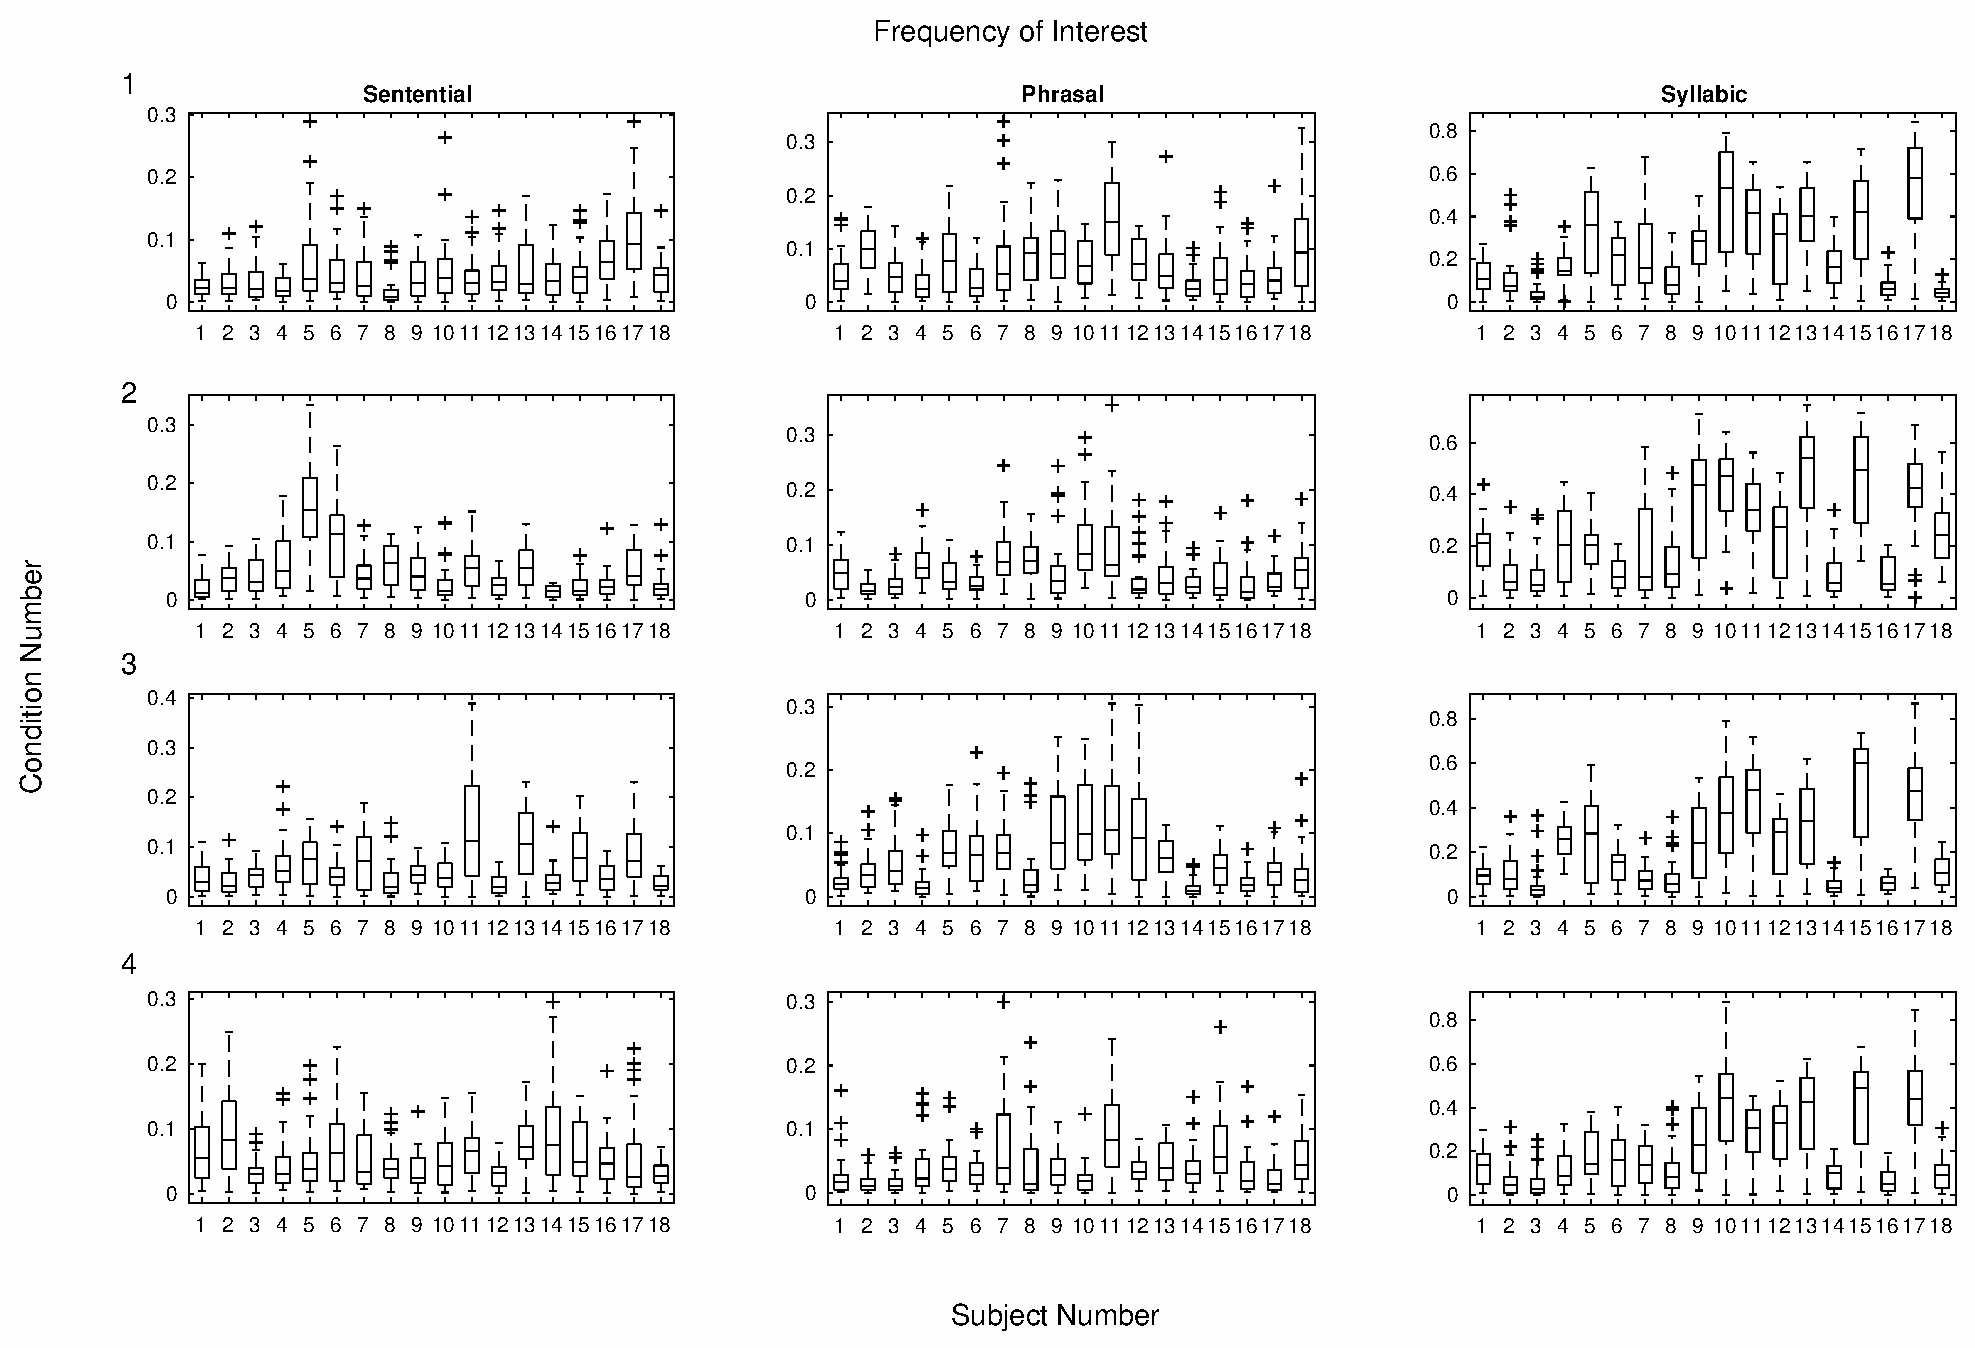
\includegraphics[width=\linewidth]{BoxPlots_per_subject.eps}
\caption{\textbf{Individual EEG responses to grammatical and ungrammatical sensical and nonsensical sentences.} Graphs showing average ITPC values at each of the frequencies of interest (1/1.28 Hz, 1/0.64 Hz, 1/0.32 Hz, \textbf{(i-iii)}, respectively) for each of the four conditions tested \textbf{(A-D)}. On the box plots the central red line indicates the median ITPC value across all electrodes for the participant, the bottom and top edges of the box indicate the 25th and 75th percentiles of the ITPC values across all electrodes. The whiskers extend to the most extreme data points not considered outliers, and the outliers are plotted individually using the '+' symbol. Stars represent statistical significance *= p$<$0.05, **= p$<$0.005, ***= p$<$0.0005.}
\label{Fig2}
\end{figure}

% Add a figure for the distibution of ITPC values

\begin{figure}[tbhp]
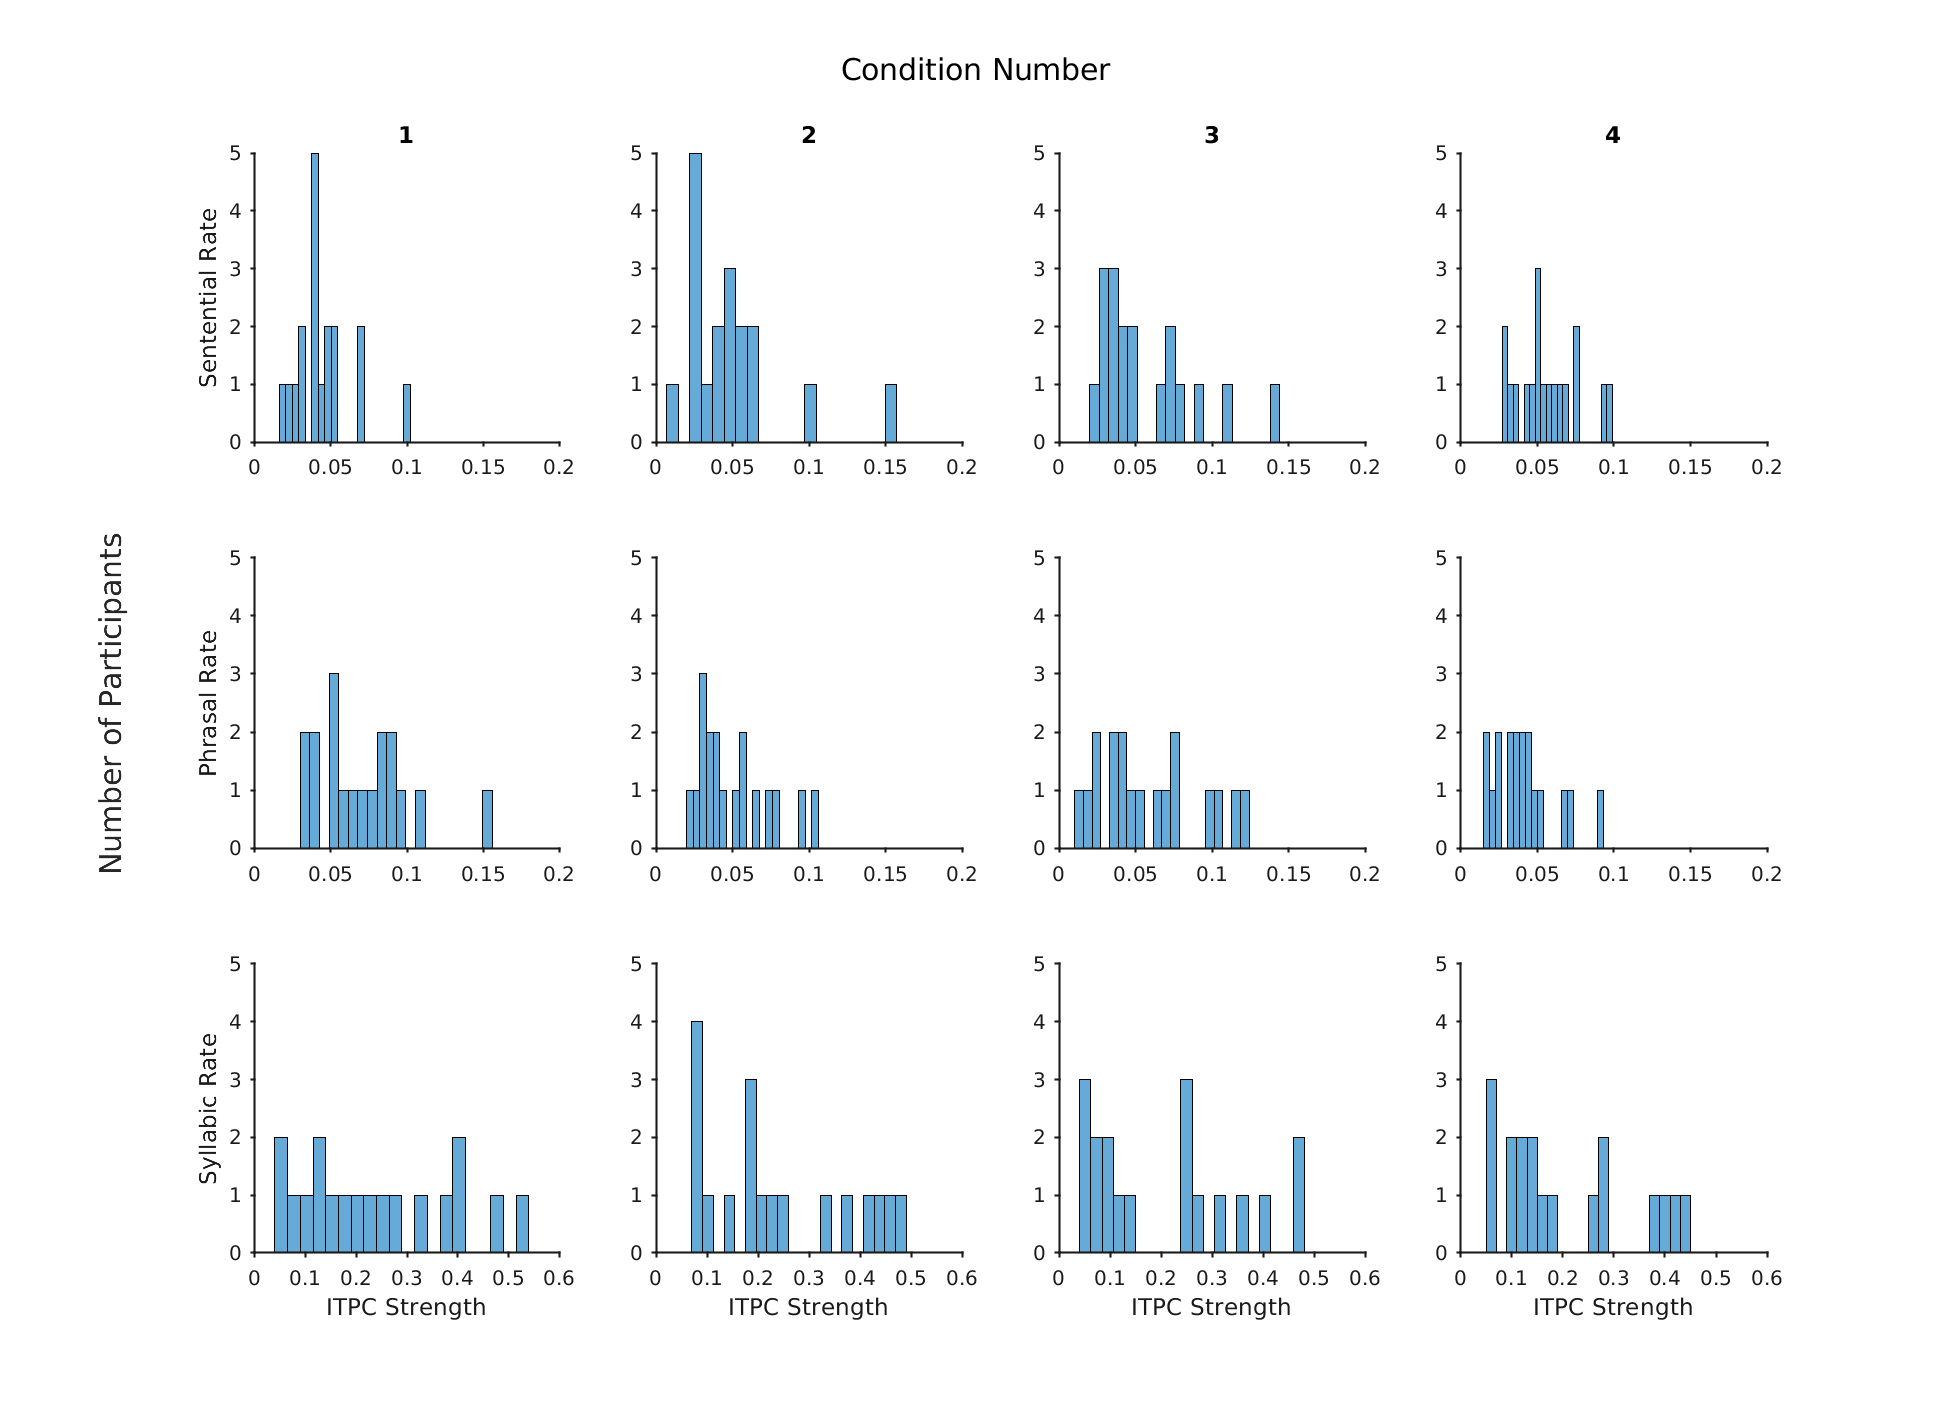
\includegraphics[width=\linewidth]{ITPC_Distributions.png}
\caption{\textbf{Distribution of ITPC values for each condition at each of the three target frequencies.} Histograms showing the distribution of ITPC values for all participants during each of the four conditions (1-4) at each of the frequencies of interest (sentential rate; 1/1.28 Hz, phrasal rate 2/1.28 Hz and syllabic rate 4/1.28 Hz).}
\label{ITPC_Distribution}
\end{figure}

The majority of participants displayed similar results to those outlined above in the grand average, but there was some variability in response at the single subject level. In condition 1, statistically significant peaks at the sentential, phrasal and syllabic frequencies are observed in 11/18,
14/18 and 17/18 participants respectively. In
condition 2, statistically significant peaks at the sentential,
phrasal and syllabic frequencies are observed in 13/18, 11/18 and
18/18 participants respectively. In condition 3,
statistically significant peaks at the sentential, phrasal and
syllabic frequencies are observed in 11/18, 12/18 and 18/18
participants respectively. In condition 4,
statistically significant peaks at the sentential, phrasal and
syllabic frequencies are observed in 14/18, 5/18 and 17/18
participants respectively.

\end{document}

